% Copyright 2004 by Till Tantau <tantau@users.sourceforge.net>.
%
% In principle, this file can be redistributed and/or modified under
% the terms of the GNU Public License, version 2.
%
% However, this file is supposed to be a template to be modified
% for your own needs. For this reason, if you use this file as a
% template and not specifically distribute it as part of a another
% package/program, I grant the extra permission to freely copy and
% modify this file as you see fit and even to delete this copyright
% notice. 

\documentclass{beamer}

\usepackage{adjustbox}
\usepackage{booktabs}
\usepackage{fullpage}
\usepackage{latexsym}
\usepackage{verbatim}
\usepackage{amsthm}
\usepackage{amssymb}
\usepackage{amsmath}
\usepackage{stackengine}
\usepackage{scalerel}
\usepackage{code,proof,amsthm,amssymb, amsmath, mathbbol}
\usepackage{proof}
\usepackage{mathpartir}
\usepackage{turnstile}
\usepackage{fancyvrb}
\usepackage{stmaryrd}
\usepackage{mathtools}
\usepackage{graphicx}
\usepackage{hyperref}
\usepackage{tikz}
\usepackage[cache=false]{minted}
\graphicspath{ {./} }
\usetikzlibrary{shapes.geometric, arrows}
\newcommand{\ms}[1]{\ensuremath{\mathsf{#1}}}
\newcommand{\irl}[1]{\mathtt{#1}}

\newcounter{rule}
\setcounter{rule}{0}
\newcommand{\rn}
  {\addtocounter{rule}{1}(\arabic{rule})}	

\newcounter{infercount}
\setcounter{infercount}{1}
\newcommand{\infern}[2]{\inferrule{#1}{#2}(\text{S}_{\arabic{infercount}}\stepcounter{infercount})}
\newcommand*\ts[2]{%
  \,\scalebox{1}[0.5]{$\sststile[ss]{\textstyle#1}{\textstyle#2}$}\,
}
\newcommand{\inferr}[2]{\inferrule{#2}{#1}}
\newcommand{\inferrr}[3]{\inferrule[#1]{#2}{#3}}
\newcommand{\paircaseabt}[4]{\irl{match_P}(#2,#3.#4)}
\newcommand{\paircasecst}[4]{\irl{match} \; #1\; \{(#2;#3) \hookrightarrow #4\}}
\newcommand{\na}[1]{\mathsf{linearCtxt}(#1)}
\newcommand{\nr}[1]{\mathsf{no\_ref}(#1)}
\newcommand{\stable}[1]{\mathsf{stable}(#1)}
\newcommand{\set}[1]{\mathsf{set}(#1)}
\newcommand{\safe}[1]{\mathsf{safe}(#1)}
\newcommand{\dist}[1]{\mathsf{disjoint}(#1)}
\newcommand{\stack}[1]{\irl{stack}(#1)}
\newcommand{\denote}[1]{\llbracket#1\rrbracket}
\newcommand{\nil}{[]}
\newcommand{\cons}[2]{\pi(#1,#2)}
\newcommand{\sharecst}[4]{\irl{share}\;#1\;\irl{as}\;#2,#3\;\irl{in}\;#4}
\newcommand{\sharecpcst}[4]{\irl{share}\;#1\;\irl{as}\;#2,#3\;\irl{in}\;#4}
\newcommand{\shareabt}[4]{\irl{share}(#1;#2,#3.#4)}
\newcommand{\ssize}[2]{\left\Vert #2 \right\Vert_{#1}}
\newcommand{\card}[1]{card(#1)}
\newcommand{\val}[1]{\irl{val}(#1)}
\newcommand{\gc}[3]{\mathsf{gc}(#1,#2,#3)}
\newcommand{\wfc}[5]{\mathsf{linearComp}(#1,#2,#3,#4,#5)}
\newcommand{\veq}[4]{#3 \sim^{#1}_{#2} #4}
\newcommand{\ctxeq}[2]{(#1) \sim (#2)}
\newcommand{\oh}[1]{\oslash(#1)}
\newcommand{\fogc}{\ms{FO}^{gc}}
\newcommand{\jan}[1]{{\color{red} [\emph{Jan: #1}]}}
\newcommand{\yue}[1]{{\color{blue} [\emph{Yue: #1}]}}
\newcommand{\gcSem}{\ensuremath{\mathcal{E}_{\ms{gc}}}}
\newcommand{\copySem}{\ensuremath{\mathcal{E}_{\ms{copy}}}}
\newtheorem{attempt}{Attempt}
\theoremstyle{definition}

% generic definitions

%\DeclareMathAccent{\colonaccent}{\mathpunct}{upright}{"3A}

% create a wavy division sign
\stackMath
\def\ccdot{\scalebox{1.15}{$\SavedStyle\cdot$}}
\def\genericform#1#2{\stackunder[#1]{\stackon[#2]{\SavedStyle\sim}{\ccdot}}{\ccdot}}
\def\altdiv{\mathrel{\ThisStyle{\mathchoice%
  {\genericform{-2.5pt}{-1.5pt}}%
  {\genericform{-2.5pt}{-1.5pt}}%
  {\genericform{-2.0pt}{-1.1pt}}%
  {\genericform{-1.4pt}{-0.8pt}}%
}}}

\newcommand{\optional}[1]{\lbrack #1\rbrack}

\newcommand{\VisibleSpace}{\mbox{\verb*/ /}}

\newcommand{\Domain}[1]{\mathop{\mathit{dom}}(#1)}
\newcommand{\Disjoint}[2]{{#1}\mathrel{\#}{#2}}
\newcommand{\NotInDom}[2]{#1\notin\Domain{#2}}
\newcommand{\NotIn}[2]{{#1}\notin{#2}}
\newcommand{\eqdef}{\mathrel{\triangleq}}
\newcommand{\isdef}{\eqdef}

\newcommand{\bnfdef}{\coloncolonequals}
\newcommand{\phantombnfdef}{\mathrel{\phantom{\bnfdef}}}
\newcommand{\bnfalt}{\mathrel{\mid}}

\newcommand{\pto}{\rightharpoonup}
\newcommand{\backsl}{\ensuremath{\backslash}}
\newcommand{\turnstile}{\ensuremath{\vdash}}
\newcommand{\twiddle}{\raisebox{-.1\height}{\texttildelow}}
%\newcommand{\twiddle}{\ensuremath{\tilde{\ }}}
\newcommand{\caret}{\ensuremath{\hat{\ }}}

\newcommand{\parens}[1]{({#1})}
\newcommand{\braces}[1]{\{{#1}\}}
\newcommand{\sqbracks}[1]{[{#1}]}
\newcommand{\ptbracks}[1]{\langle #1\rangle}
\newcommand{\brackets}[1]{\ptbracks{#1}}
\newcommand{\corners}[1]{\ulcorner #1\urcorner}
\newcommand{\dblptbracks}[1]{\langle\!\langle #1\rangle\!\rangle}
\newcommand{\dblsqbracks}[1]{[\![ #1]\!]}

\newcommand{\kw}[1]{\ensuremath{\mathtt{#1}}}
\newcommand{\kwop}[1]{\ensuremath{\mathop{\mathtt{#1}}}}
\newcommand{\kwbin}[1]{\ensuremath{\mathbin{\mathtt{#1}}}}

\newcommand{\cdcolon}{\kwbin{:}}
\newcommand{\cdcoloncolon}{\kwbin{::}}
\newcommand{\cdcomma}{\kw{,}}
\newcommand{\cdperiod}{\kw{.}}
\newcommand{\cddot}{\cdperiod}
\newcommand{\cddotdot}{\kw{{.}{.}}}
\newcommand{\cdsemi}{\kw{;}}
\newcommand{\cdbar}{\kwbin{|}} %|
\newcommand{\cdatsign}{\kw{@}}
\newcommand{\cdunderscore}{\kw{\_}}
\newcommand{\cdsharp}{\kw{\#}}
\newcommand{\cddollar}{\kw{\$}}
\newcommand{\cdtwiddle}{\kw{\~}}
\newcommand{\cdhat}{\kw{\^{ }}}
\newcommand{\cdstar}{\kw{*}}
\newcommand{\cdamper}{\kw{\&}}

\newcommand{\seq}[2]{{#2}_1,\dots,{#2}_{#1}}
\newcommand{\zeq}[2]{{#2}_0,\dots,{#2}_{#1-1}}
\newcommand{\seqsep}[3]{{#3}_1\mathbin{#1}\dots\mathbin{#1}{#3}_{#2}}
\newcommand{\zeqsep}[3]{{#3}_0\mathbin{#1}\dots\mathbin{#1}{#3}_{#2-1}}

\newcommand{\abs}[1]{\lvert#1\rvert}

\newcommand{\cdparens}[1]{\kw{(}{#1}\kw{)}}
\newcommand{\cdnoparens}[1]{#1}
\newcommand{\noparens}[1]{#1}
\newcommand{\cdcdc}{\kw{,}\dots\kw{,}}
\newcommand{\cdcds}{\kw{;}\dots\kw{;}}
\newcommand{\cdseq}[2]{#2_{1}\cdcdc #2_{#1}}
\newcommand{\cdzeq}[2]{#2_{0}\cdcdc #2_{#1-1}}
\newcommand{\cdsseq}[2]{#2_{1}\cdcds #2_{#1}}
\newcommand{\cdszeq}[2]{#2_{0}\cdcds #2_{#1-1}}
\newcommand{\cdpseq}[4]{{#3}_{1}{#2}{#4}_{1}\cdcdc{#3}_{#1}{#2}{#4}_{#1}}
\newcommand{\cdpzeq}[4]{{#3}_{0}{#2}{#4}_{0}\cdcdc{#3}_{#1-1}{#2}{#4}_{#1-1}}
\newcommand{\cdsqbracks}[1]{\kw{[}{#1}\kw{]}}
\newcommand{\cdptbracks}[1]{\kw{<}{#1}\kw{>}}
\newcommand{\cdrdbracks}[1]{\cdparens{#1}}
\newcommand{\cdbrackets}[1]{\cdptbracks{#1}}
\newcommand{\cdbraces}[1]{\kw{\{}{#1}\kw{\}}}
\newcommand{\cdcurlbracks}[1]{\cdbraces{#1}}

\newcommand{\IsType}[1]{\JPost{#1}{\textsf{type}}}
\newcommand{\IsTp}[1]{\IsType{#1}}
\newcommand{\IsKd}[1]{\JPost{#1}{\textsf{kind}}}
\newcommand{\EqTy}[2]{{#1}\equiv{#2}}
\newcommand{\EqTp}[2]{\EqTy{#1}{#2}}
\newcommand{\EqKd}[2]{{#1}\equiv{#2}}
\newcommand{\IsOf}[2]{{#1}\mathrel{:}{#2}}
\newcommand{\IsOfP}[2]{\IsOf{#1}{#2}}
\newcommand{\IsOfM}[2]{{#1}\mathrel{\altdiv}{#2}}
\newcommand{\IsOfMW}[3]{{#1}\mathrel{\altdiv}{#2}\mathrel{@}{#3}}
\newcommand{\IsOfW}[3]{{#1}\mathbin{:}{#2}\mathbin{@}{#3}}
\newcommand{\Has}[2]{{#1}\mathbin{\twiddle}{#2}}
\newcommand{\HasW}[3]{{#1}\mathbin{\twiddle}{#2}\mathbin{@}{#3}}
\newcommand{\IsOfKd}[2]{{#1}\mathrel{\coloncolon}{#2}}
\newcommand{\TightIsOfKd}[2]{{#1}\mathbin{\coloncolon}{#2}}
\newcommand{\TightIsOf}[2]{{#1}\mathbin{:}{#2}}
\newcommand{\NIsOfKd}[2]{{#1}\mathrel{\Uparrow}{#2}}
\newcommand{\CIsOfKd}[2]{{#1}\mathrel{\Downarrow}{#2}}
\newcommand{\EqOfKd}[3]{{#1}\mathrel{\equiv}{#2}\mathrel{\coloncolon}{#3}}
\newcommand{\IsVal}[1]{\JPost{#1}{\textsf{val}}}
\newcommand{\IsntVal}[1]{\JPost{#1}{\mathop{\neg}\textsf{val}}}
\newcommand{\LIsVal}[2]{\JPost{#2}{\textsf{val}_{#1}}}
\newcommand{\IsErr}[1]{\JPost{#1}{\textsf{err}}}
\newcommand{\IsOK}[1]{\JPost{#1}{\textsf{ok}}}
\newcommand{\LIsOK}[2]{\JPost{#2}{\textsf{ok}_{#1}}}

\newcommand{\IsOfSy}[2]{{#1}\uparrow{#2}}
\newcommand{\IsOfAn}[2]{{#1}\downarrow{#2}}

\newcommand{\IsOpnVal}[2]{{#1}\vdash\IsVal{#2}}

\newcommand{\IsMobile}[1]{\JPost{#1}{\textsf{mobile}}}

\newcommand{\DefEqv}[3]{\IsOf{{#1}\equiv{#2}}{#3}}
\newcommand{\IsDefEqvCl}[3]{\DefEqv{#1}{#2}{#3}}
\newcommand{\IsDefEqv}[4]{{#1}\vdash\DefEqv{#2}{#3}{#4}}
\newcommand{\IsDefEqvU}[3]{{#1}\vdash{#2}\equiv{#3}}
\newcommand{\DefEqvU}[2]{{#1}\equiv{#2}}

\newcommand{\JPre}[2]{{#2}\;{#1}}
\newcommand{\JPPre}[2]{{#2}\parens{#1}}
\newcommand{\JPost}[2]{{#1}\;{#2}}
\newcommand{\JPPost}[2]{\parens{#1}\;{#2}}
%\newcommand{\JPostTight}[2]{{#1}\,{#2}}
\newcommand{\JInfix}[3]{{#1}\mathrel{#2}{#3}}

% \newcommand{\imode}{{\forall}}
% \newcommand{\omode}{{\exists}}
% \newcommand{\oumode}{{\exists!}}
% \newcommand{\opmode}{{\exists^{\leq 1}}}

%\newcommand{\tytransto}[2]{{#1}\leadsto {#2}}
%\newcommand{\extransto}[2]{{#1}\leadsto {#2}}
% \newcommand{\extranstostacked}[2]{%
%   \begin{array}[c]{c}
%     {#1} \\
%     \leadsto \\
%     {#2}
%   \end{array}
% }

% finite functions
\newcommand{\ff}[1]{\braces{#1}}
\newcommand{\pairff}[2]{{#1}\mathbin{\hookrightarrow}{#2}}
\newcommand{\empff}{\emptyset}
\newcommand{\singff}[2]{\ff{\pairff{#1}{#2}}}
\newcommand{\combff}[2]{#1\mathbin{\otimes}#2}
\newcommand{\extff}[3]{\combff{#1}{\singff{#2}{#3}}}
\newcommand{\varextff}[3]{\combff{#1}{\pairff{#2}{#3}}}
\newcommand{\appff}[2]{{#1}\parens{#2}}
\newcommand{\explff}[3]{\ff{\pairff{{#2}_{0}}{{#3}_{0}},\dots,\pairff{{#2}_{{#1}-1}}{{#3}_{{#1}-1}}}}
\newcommand{\varexplff}[3]{\pairff{#2_{1}}{#3_{1}},\dots,\pairff{#2_{#1}}{#3_{#1}}}
\newcommand{\domff}[1]{\Domain{#1}}
\newcommand{\disjff}[2]{\domff{#1}\cap\domff{#2}=\emptyset}
\newcommand{\genff}[3]{\ff{{#2}\mathbin{\hookrightarrow}{#3}}_{{#2}\in{#1}}}

% families of judgments
\newcommand{\FamInst}[2]{{#1}\,[{#2}]}
\newcommand{\JFam}[3]{\FamInst{\JPPre{#3}{#1}}{#2}}

% language names
\newcommand{\textbsf}[1]{\textbf{\textsf{#1}}}
\newcommand{\Lang}[1]{\textbsf{#1}}

\newcommand{\calA}{\mathcal{A}}
\newcommand{\calB}{\mathcal{B}}
\newcommand{\calC}{\mathcal{C}}
\newcommand{\calE}{\mathcal{E}}
\newcommand{\calG}{\mathcal{G}}
\newcommand{\calI}{\mathcal{I}}
\newcommand{\calL}{\mathcal{L}}
\newcommand{\calO}{\mathcal{O}}
\newcommand{\calP}{\mathcal{P}}
\newcommand{\calQ}{\mathcal{Q}}
\newcommand{\calR}{\mathcal{R}}
\newcommand{\calS}{\mathcal{S}}
\newcommand{\calU}{\mathcal{U}}
\newcommand{\calV}{\mathcal{V}}
\newcommand{\calX}{\mathcal{X}}
\newcommand{\calY}{\mathcal{Y}}

% general judgment
\newcommand{\vargen}{\mathrel{\vert}}
\newcommand{\symgen}{\mathrel{\Vert}}

%%% Local Variables: 
%%% mode: latex
%%% TeX-master: "book"
%%% End: 

% generic symbols
\newcommand{\IsSymb}[1]{\JPost{#1}{\mathsf{sym}}}
\newcommand{\IsSym}[1]{\IsSymb{#1}}
\newcommand{\Diff}[2]{{#1}\not={#2}}
\newcommand{\DiffSymb}[2]{\IsSymb{\Diff{#1}{#2}}}

% strings
\newcommand{\IsChar}[1]{\JPost{#1}{\mathsf{char}}}
\newcommand{\IsString}[2]{\JPost{#2}{\mathsf{str}_{#1}}}
\newcommand{\IsStr}[1]{\JPost{#1}{\mathsf{str}}}
\newcommand{\IsCharStr}[1]{\IsString{\mathsf{char}}{#1}}
\newcommand{\NullString}{\epsilon}
\newcommand{\ConsString}[2]{{#1}\cdot{#2}}
\newcommand{\SingString}[1]{\ConsString{#1}{\NullString}}
\newcommand{\SingStringStar}[1]{#1}
\newcommand{\ConcString}[2]{{#1}\mathbin{\hat{\ }}{#2}}
\newcommand{\ConcStringStar}[2]{{#1}\,{#2}}
\newcommand{\IsConc}[3]{\JPPre{#1;#2;#3}{\mathsf{conc}}}
\newcommand{\ConcIs}[3]{\ConcString{#1}{#2}={#3}}
\newcommand{\IsEqStr}[2]{{#1}={#2}}
\newcommand{\LenIs}[2]{|{#1}|={#2}}

% permutations
\newcommand{\IdPerm}{\mathop{\mathit{id}}}
\newcommand{\SwapPerm}[2]{\sqbracks{{#1}\leftrightarrow{#2}}}
\newcommand{\CompPerm}[2]{{#1}\circ{#2}}

% sorts
\newcommand{\Sort}[1]{\textsf{#1}}
\newcommand{\Op}[1]{\kw{#1}}
\newcommand{\Ar}[2]{\parens{#1}{#2}}
\newcommand{\Vl}[2]{\noparens{#1}\cddot{#2}}
\newcommand{\OpInst}[2]{{#1}\cdsqbracks{#2}}

\newcommand{\ExprSort}{\Sort{Exp}}
\newcommand{\TypeSort}{\Sort{Typ}}
\newcommand{\RefSort}{\Sort{Ref}}

% asts
\newcommand{\IsOpn}[1]{\JPost{#1}{\mathsf{opn}}}

\newcommand{\OpAST}[2]{{#1}\cdparens{#2}}
\newcommand{\AbsAST}[2]{{#1}\cddot{#2}}

\newcommand{\BvarABG}[1]{\OpInst{\kw{bv}}{#1}}
\newcommand{\AbsABG}[1]{\cddot{#1}}

\newcommand{\OpABT}[2]{{#1}\cdparens{#2}}
\newcommand{\OpABTp}[3]{{#1}\cdbraces{#2}\cdparens{#3}}
\newcommand{\OpABTpp}[4]{{#1}\cdbraces{#2}\cdbraces{#3}\cdparens{#4}}
\newcommand{\OpABTn}[2]{{#1}\cdbraces{#2}}
\newcommand{\AbsABT}[2]{{#1}\cddot{#2}}
\newcommand{\SymABT}[2]{\AbsABT{#1}{#2}}

\newcommand{\ListABT}[2]{{#1}\cdsemi\dots\cdsemi{#2}}
\newcommand{\SeqABT}[2]{\ListABT{{#2}_1}{{#2}_{#1}}}
\newcommand{\ZeqABT}[2]{\ListABT{{#2}_0}{{#2}_{#1}}}

% size

\newcommand{\SzABTn}[3]{\mathop{\mathsf{sz}}(\IsABTn{#1}{#2})=#3}

% apartness, occurrence
\newcommand{\IsFree}[2]{{#1}\in{#2}}
\newcommand{\IsntFree}[2]{{#1}\notin{#2}}
\newcommand{\IsApart}[2]{{#1}\notin{#2}}
\newcommand{\Apart}[2]{\IsApart{#1}{#2}}

\newcommand{\Swap}[3]{\mathop{\SwapPerm{#1}{#2}}{#3}}
\newcommand{\SwapIs}[4]{\Swap{#1}{#2}{#3}={#4}}

%\newcommand{\PermAct}[2]{{#1}\mathbin{\cdot}{#2}}
\newcommand{\PermAct}[2]{\widehat{#1}\parens{#2}}
\newcommand{\PermActIs}[3]{\PermAct{#1}{#2}={#3}}
\newcommand{\PermActIsAST}[3]{\IsAST{\PermActIs{#1}{#2}{#3}}}

% \newcommand{\IsVar}[1]{\JPost{#1}{\mathsf{var}}}

\newcommand{\Subst}[3]{\sqbracks{{#1}\mathord{/}{#2}}{#3}}
\newcommand{\SubstIs}[4]{\Subst{#1}{#2}{#3}\mathbin{=}{#4}}
\newcommand{\SubstIsAST}[4]{\IsAST{\SubstIs{#1}{#2}{#3}{#4}}}
\newcommand{\SubstIsABTn}[5]{\IsABTn{\SubstIs{#1}{#2}{#3}{#4}}{#5}}
\newcommand{\SubstIsABT}[4]{\IsABT{\SubstIsAbt{#1}{#2}{#3}{#4}}}

\newcommand{\AlphaEq}[2]{{#1}=_\alpha{#2}}
\newcommand{\AlphaEqABTn}[3]{\IsABTn{\AlphaEq{#1}{#2}}{#3}}
\newcommand{\AlphaEqABT}[2]{\IsABT{\AlphaEq{#1}{#2}}}
\newcommand{\NotAlphaEq}[2]{{#1}\not=_\alpha{#2}}

%%% Local Variables: 
%%% mode: latex
%%% TeX-master: "book"
%%% End: 

\newcommand{\FunEvalsTo}[3]{{#1}\mathrel{\Downarrow'}\AbsABT{#2}{#3}}
\newcommand{\FunEvalsToHO}[3]{{#2}\vargen \fappabt{#1}{#2}\evalsto{#3}}

\newcommand{\arrtyabt}[2]{\OpABT{\cd{arr}}{#1;#2}}
\newcommand{\arrtycst}[2]{{#1}\mathrel{\to}{#2}}
\newcommand{\lamabt}[3]{\OpABTp{\cd{lam}}{#1}{\AbsABT{#2}{#3}}}
\newcommand{\lamcst}[3]{\mathop{\lambda}\cdparens{\TightIsOf{#2}{#1}}\,{#3}}
\newcommand{\appabt}[2]{\OpABT{\cd{ap}}{#1;#2}}
\newcommand{\appcst}[2]{{#1}\cdparens{#2}}

\newcommand{\letabt}[4]{\OpABTp{\cd{let}}{#1}{#2;\AbsABT{#3}{#4}}}
\newcommand{\letcst}[4]{\kwop{let}\TightIsOf{#3}{#1}\kwop{be}{#2}\kwop{in}{#4}}
\newcommand{\uletabt}[3]{\kwop{let}{(#2;\AbsABT{#1}{#3})}}
\newcommand{\uletcst}[3]{\kwop{let}{#2}\kwop{be}{#1}\kwop{in}{#3}}

\newcommand{\fdefabt}[6]{\OpABTp{\cd{fun}}{#1;#2}{\AbsABT{#3}{#4};\AbsABT{#5}{#6}}}
\newcommand{\fdefcst}[6]{\kwop{fun}{#5}\TightIsOf{\cdparens{\TightIsOf{#3}{#1}}}{#2}\mathbin{\cd{=}}{#4}\kwop{in}{#6}}
\newcommand{\fappabt}[2]{\OpABTp{\cd{apply}}{#1}{#2}}
\newcommand{\fappcst}[2]{#1\cdparens{#2}}
\newcommand{\fsubst}[3]{\dblsqbracks{#1\mathord{/}#2}{#3}}


%%% Local Variables: 
%%% mode: latex
%%% TeX-master: "book"
%%% End: 

\newcommand{\LangPCF}{\textbsf{PCF}}

\newcommand{\genrecabt}[3]{\OpABTp{\cd{fix}}{#1}{\AbsABT{#2}{#3}}}
\newcommand{\genreccst}[3]{\kwop{fix}{#2}\cdcolon{#1}\kwop{is}{#3}}
\newcommand{\sgenreccst}[2]{\kwop{fix}{#1}\kwop{is}{#2}}

\newcommand{\bddrecabt}[4]{\OpABTp{\cd{fix}^{#1}}{#2}{\AbsABT{#3}{#4}}}
\newcommand{\bddreccst}[4]{\mathop{\cd{fix}^{#1}}{#3}\cdcolon{#2}\kwop{is}{#4}}

\newcommand{\parrtyabt}[2]{\OpABT{\cd{parr}}{#1;#2}}
\newcommand{\parrtycst}[2]{{#1}\mathbin{\rightharpoonup}{#2}}
\newcommand{\pappabt}[2]{\OpABT{\cd{ap}}{#1;#2}}
\newcommand{\pappcst}[2]{\appcst{#1}{#2}}

\newcommand{\funabt}[5]{\OpABTp{\cd{fun}}{#1;#2}{\AbsABT{#3}{\AbsABT{#4}{#5}}}}
\newcommand{\funcst}[5]{\kwop{fun}{#3}\cdparens{{#4}{\cdcolon}{#1}}{\cdcolon}{#2}\kwop{is}{#5}}

\newcommand{\empenv}{\bullet}
\newcommand{\extenv}[3]{{#1},{#2}{=}{#3}}

\newcommand{\expclo}[1]{\widehat{#1}}
\newcommand{\expclois}[2]{\expclo{#1}{=}{#2}}
\newcommand{\expenv}[2]{\widehat{#1}\parens{#2}}
\newcommand{\expenvis}[3]{\expenv{#1}{#2}{=}{#3}}

\newcommand{\cutoff}[2]{{#1}^{(#2)}}

%\newcommand{\Replace}[3]{\sqbracks{#2\mathbin{\leftarrow}#1}{#3}}

\newcommand{\lnattyabt}{\cd{lnat}}
\newcommand{\lnattycst}{\lnattyabt}
\newcommand{\lsuccabt}[2]{\OpABT{\cd{succ}}{\AbsABT{#1}{#2}}}
\newcommand{\lsucccst}[2]{{#1}\kwbin{is}\succcst{#2}}

%%% Local Variables: 
%%% mode: plain-tex
%%% TeX-master: "book"
%%% End: 

\newcommand{\unittyabt}{\kw{unit}}
\newcommand{\unittycst}{\kw{unit}}
\newcommand{\unittycstm}{\top}
\newcommand{\prodtyabt}[2]{\OpABT{\kw{prod}}{#1;#2}}
\newcommand{\prodtycst}[2]{{#1}\times{#2}}

\newcommand{\pprodtycst}[2]{{#1}\otimes{#2}}
\newcommand{\ppairexabt}[2]{\OpABT{\kw{fuse}}{#1;#2}}
\newcommand{\ppairexcst}[2]{{#1}\otimes{#2}}
\newcommand{\splitexabt}[4]{\OpABT{\kw{split}}{{#1};\AbsABT{#2,#3}{#4}}}
\newcommand{\splitexcst}[4]{\kw{split}\,{#1}\,\kw{as}\,\ppairexcst{#2}{#3}\,\kw{in}\,{#4}}
\newcommand{\checkexabt}[2]{\OpABT{\kw{check}}{#1;#2}}
\newcommand{\checkexcst}[2]{\kw{check}\,{#1}\,\kw{as}\,\unitexcst\,\kw{in}\,{#2}}

\newcommand{\unitexabt}{\kw{triv}}
\newcommand{\unitexcst}{\langle\rangle}
\newcommand{\pairexabt}[2]{\OpABT{\kw{pair}}{#1;#2}}
\newcommand{\pairexcst}[2]{\langle #1, #2\rangle}
\newcommand{\projexabt}[2]{\OpABT{\OpInst{\kw{pr}}{#2}}{#1}}
\newcommand{\fstexabt}[1]{\projexabt{#1}{\kw{l}}}
\newcommand{\sndexabt}[1]{\projexabt{#1}{\kw{r}}}
\newcommand{\projexcst}[2]{{#1}\mathbin\cdot{#2}}
\newcommand{\fstexcst}[1]{\projexcst{#1}{\kw{l}}}
\newcommand{\sndexcst}[1]{\projexcst{#1}{\kw{r}}}

\newcommand{\dgenprodcst}[1]{\brackets{#1}}
\newcommand{\dgentuplecst}[1]{\brackets{#1}}
\newcommand{\genprodabt}[3]{\OpABT{\kw{prod}}{\genff{#1}{#2}{#3}}}
\newcommand{\vargenprodcst}[3]{\prod_{{#2}\in{#1}}{#3}}
\newcommand{\genprodcst}[3]{\dgenprodcst{#3}_{#2\in #1}}
\newcommand{\gentupleabt}[3]{\OpABT{\kw{tpl}}{\genff{#1}{#2}{#3}}}
\newcommand{\gentuplecst}[3]{\dgentuplecst{#3}_{{#2}\in{#1}}}
\newcommand{\lgentuplescst}[3]{\gentuplecst{#1}{#2}{\fldexcst{#2}{#3}}}
\newcommand{\genprojabt}[3]{\projexabt{#3}{#2}}
\newcommand{\genprojcst}[3]{\projexcst{#3}{#2}}
\newcommand{\genprodcstgen}[3]{\dgenprodcst{\varexplff{#1}{#2}{#3}}}
\newcommand{\gentuplecstgen}[3]{\dgentuplecst{\varexplff{#1}{#2}{#3}}}

\newcommand{\rcdtycst}[1]{\dgenprodcst{#1}}
\newcommand{\rcdexcst}[1]{\dgentuplecst{#1}}
\newcommand{\fldtycst}[2]{\pairff{#1}{#2}}
\newcommand{\fldexcst}[2]{\pairff{#1}{#2}}
\newcommand{\fldselexcst}[2]{\projexcst{#2}{#1}}


%%% Local Variables: 
%%% mode: latex
%%% TeX-master: "book"
%%% End: 

\newcommand{\casesepcst}{\ensuremath{\mathbin{\cdbar}}}
\newcommand{\casebrcst}{\ensuremath{\mathbin{\hookrightarrow}}}


\newcommand{\voidtyabt}{\kw{void}}
\newcommand{\voidtycst}{\voidtyabt}
\newcommand{\voidtycstm}{\bot}
\newcommand{\abortexcst}[2]{\OpABT{\kw{abort}}{#2}}
\newcommand{\nullcaseexcst}[2]{\abortexcst{#1}{#2}}
\newcommand{\sumtyabt}[2]{\OpABT{\kw{sum}}{#1;#2}}
\newcommand{\sumtycst}[2]{{#1}\mathbin{+}{#2}}
\newcommand{\abortexabt}[2]{\OpABTp{\kw{abort}}{#1}{#2}}
\newcommand{\nullcaseexabt}[2]{\abortexabt{#1}{#2}}
\newcommand{\inexabt}[3]{\OpABTp{\OpInst{\kw{in}}{#2}}{#1}{#3}}
\newcommand{\inexcst}[3]{{#2}\mathbin{\cdot}{#3}}
\newcommand{\inlexabt}[3]{\inexabt{#1;#2}{\kw{l}}{#3}}
\newcommand{\inlexcst}[2]{\inexcst{}{\kw{l}}{#2}}
\newcommand{\varinlexcst}[3]{\inlexcst{}{#3}}
\newcommand{\inrexabt}[3]{\inexabt{#1;#2}{\kw{r}}{#3}}
\newcommand{\inrexcst}[2]{\inexcst{}{\kw{r}}{#2}}
\newcommand{\varinrexcst}[3]{\inrexcst{}{#3}}
\newcommand{\caseexabt}[7]{\OpABT{\kw{case}}{#1;\AbsABT{#2}{#4};\AbsABT{#5}{#7}}}
\newcommand{\caseexcst}[7]{\kwop{case}{#1}\,\cdbraces{\inlexcst{}{#2}\casebrcst{#4}\casesepcst\inrexcst{}{#5}\casebrcst{#7}}}

\newcommand{\dgensumcst}[1]{\cdsqbracks{#1}}
\newcommand{\gensumabt}[3]{\OpABT{\kw{sum}}{\genff{#1}{#2}{#3}}}
\newcommand{\vargensumcst}[3]{\sum_{{#2}\in{#1}}{#3}}
\newcommand{\gensumcst}[3]{\dgensumcst{#3}_{#2\in #1}}
\newcommand{\geninjabt}[3]{\inexabt{#1}{#2}{#3}}
\newcommand{\geninjcst}[3]{\inexcst{}{#2}{#3}}
\newcommand{\gencaseabt}[5]{\OpABT{\kw{case}}{#2;\genff{#1}{#3}{\AbsABT{#4}{#5}}}}
\newcommand{\gencasecst}[5]{\kwop{case}{#2}\,\cdbraces{\geninjcst{#1}{#3}{#4}\casebrcst{#5}}_{{#3}\in{#1}}}
\newcommand{\dgencasecst}[3]{\kwop{case}{#2}\,\cdbraces{#3}}
\newcommand{\gensumcstgen}[3]{\dgensumcst{\varexplff{#1}{#2}{#3}}}
\newcommand{\gencasecstgen}[5]{\dgencasecst{}{#2}{\geninjcst{}{#3_1}{#4_1}\casebrcst{#5_1}\casesepcst\dots\casesepcst\geninjcst{}{#3_{#1}}{#4_{#1}}\casebrcst{#5_{#1}}}}

\newcommand{\booltyabt}{\kw{bool}}
\newcommand{\booltycst}{\booltyabt}
\newcommand{\trexabt}{\kw{true}}
\newcommand{\trexcst}{\trexabt}
\newcommand{\faexabt}{\kw{false}}
\newcommand{\faexcst}{\faexabt}
\newcommand{\ifexabt}[3]{\OpABT{\kw{if}}{#1;#2;#3}}
\newcommand{\ifexcst}[3]{\kwop{if}{#1}\kwop{then}{#2}\kwop{else}{#3}}

\newcommand{\opttyabt}[1]{\OpABT{\kw{opt}}{#1}}
\newcommand{\opttycst}[1]{{#1}\,\kw{opt}}
\newcommand{\noneexabt}{\kw{null}}
\newcommand{\noneexcst}{\noneexabt}
\newcommand{\someexabt}[1]{\OpABT{\kw{just}}{#1}}
\newcommand{\someexcst}[1]{\someexabt{#1}}
\newcommand{\whichexabt}[5]{\OpABTpp{\kw{ifnull}}{#4}{#2;\AbsABT{#3}{#5}}{#1}}
\newcommand{\whichexcst}[5]{\kwop{which}{#1}\,\cdbraces{\noneexcst\casebrcst{#2}\casesepcst\someexcst{#3}\casebrcst{#5}}}

\newcommand{\vartycst}[1]{\dgensumcst{#1}}
\newcommand{\alttycst}[2]{\pairff{#1}{#2}}
\newcommand{\varinjexcst}[2]{\geninjcst{}{#1}{#2}}

\newcommand{\altcst}[4]{\geninjcst{}{#1}{#3}\casebrcst{#4}}
\newcommand{\varcaseexcst}[2]{\kwop{case}{#1}\,\cdbraces{#2}}

\newcommand{\suitty}{\kw{suit}}
\newcommand{\casesuit}[5]{\kwop{case}{#1}\,\cdbraces{\clubsuit\casebrcst{#2}\casesepcst\diamondsuit\casebrcst{#3}\casesepcst\heartsuit\casebrcst{#4}\casesepcst\spadesuit\casebrcst{#5}}}
\newcommand{\casesuitcst}[5]{\varcaseexcst{#1}{\altcst{\kw{clubs}}{#1}{\unittycst}{\_}{#2}}\casesepcst\altcst{\kw{diamonds}}{\unittycst}{\_}{#3}\casesepcst\altcst{\kw{hearts}}{\unittycst}{\_}{#4}\casesepcst\altcst{\kw{spades}}{\unittycst}{\_}{#5}}

%\newcommand{\chartycst}{\kw{char}}
\newcommand{\codech}[1]{\OpABT{\kw{codech}}{#1}}
\newcommand{\chcode}[1]{\OpABT{\kw{chcode}}{#1}}
\newcommand{\chcodetycst}{\kw{chcode}}

\newcommand{\sigtyabt}{\kw{signal}}
\newcommand{\sigtycst}{\kw{signal}}

%%% Local Variables: 
%%% mode: latex
%%% TeX-master: "book"
%%% End: 

\newcommand{\LangM}{\textbsf{M}}    % Mendler's M

\newcommand{\indrecnatcst}[4]{\kw{rec}_{\nattycst}\cdparens{\AbsABT{#2}{#3};{#4}}}
\newcommand{\indinnatcst}[1]{\kw{fold}_{\nattycst}\cdparens{#1}}

\newcommand{\choicecst}{\ensuremath{\mathbin{\cdamper}}}

\newcommand{\streamtycst}{\kw{stream}}
\newcommand{\strgencst}[4]{\kwop{strgen}{#2}\,\kw{is}\,{#1}\,\kw{in}\,\cdptbracks{\pairff{\kw{hd}}{#3}\cdcomma\pairff{\kw{tl}}{#4}}}
\newcommand{\shdcst}[1]{\OpABT{\kw{hd}}{#1}}
\newcommand{\stlcst}[1]{\OpABT{\kw{tl}}{#1}}
\newcommand{\stlncst}[2]{\OpABT{\kw{tl}^{(#1)}}{#2}}
\newcommand{\seqtycst}{\kw{seq}}

\newcommand{\itreetycst}{\kw{itree}}
\newcommand{\iviewcst}[1]{\OpABT{\kw{view}}{#1}}
\newcommand{\itreegencst}[3]{\kwop{itgen}{#2}\,\kw{is}\,{#1}\,\kw{in}\,{#3}}

\newcommand{\coigenstrcst}[3]{\kw{gen}_{\streamtycst}\cdparens{\AbsABT{#1}{#2};{#3}}}
\newcommand{\coioutstrcst}[1]{\kw{unfold}_{\streamtycst}\cdparens{#1}}

\newcommand{\indtyabt}[2]{\OpABT{\kw{ind}}{\AbsABT{#1}{#2}}}
\newcommand{\indtycstg}[1]{\OpABT{\mu}{#1}}
\newcommand{\indtycst}[2]{\indtycstg{\AbsABT{#1}{#2}}}

\newcommand{\indinabt}[3]{\OpABTp{\kw{fold}}{\AbsABT{#1}{#2}}{#3}}
\newcommand{\indincstg}[2]{\OpABT{\kw{fold}_{#1}}{#2}}
\newcommand{\indincst}[3]{\indincstg{\AbsABT{#1}{#2}}{#3}}
\newcommand{\sindincst}[1]{\indincstg{}{#1}} % short form
\newcommand{\indrecabt}[5]{\OpABTp{\kw{rec}}{\AbsABT{#1}{#2}}{\AbsABT{#3}{#4};{#5}}}
\newcommand{\indreccstg}[3]{\OpABT{\kw{rec}_{#1}}{#2;#3}}
\newcommand{\indreccst}[5]{\indreccstg{}{\AbsABT{#3}{#4}}{#5}}

\newcommand{\coityabt}[2]{\OpABT{\kw{coi}}{\AbsABT{#1}{#2}}}
\newcommand{\coitycstg}[1]{\OpABT{\nu}{#1}}
\newcommand{\coitycst}[2]{\coitycstg{\AbsABT{#1}{#2}}}

\newcommand{\coioutabt}[3]{\OpABTp{\kw{unfold}}{\AbsABT{#1}{#2}}{#3}}
\newcommand{\coioutcstg}[2]{\OpABT{\kw{unfold}_{#1}}{#2}}
\newcommand{\coioutcst}[3]{\coioutcstg{\AbsABT{#1}{#2}}{#3}}
\newcommand{\scoioutcst}[1]{\coioutcstg{}{#1}} % short form
\newcommand{\coigenabt}[5]{\OpABTp{\kw{gen}}{\AbsABT{#1}{#2}}{\AbsABT{#3}{#4};{#5}}}
\newcommand{\coigencstg}[3]{\OpABT{\kw{gen}_{#1}}{#2;#3}}
\newcommand{\coigencst}[5]{\coigencstg{}{\AbsABT{#3}{#4}}{#5}}

\newcommand{\conattycst}{\kw{conat}}
\newcommand{\omegaexcst}{\omega}

\newcommand{\naticst}{\nattycst}
\newcommand{\natfcst}{\conattycst}

\newcommand{\listtyabt}[1]{\OpABT{\kw{list}}{#1}}
\newcommand{\listtycst}[1]{{#1}\,\kw{list}}
\newcommand{\natlisttyabt}{\kw{natlist}}
\newcommand{\natlisttycst}{\kw{natlist}}
\newcommand{\nilexabt}{\kw{nil}}
\newcommand{\nilexcst}{\nilexabt}
\newcommand{\consexabt}[2]{\OpABT{\kw{cons}}{#1;#2}}
\newcommand{\consexcst}[2]{\consexabt{#1}{#2}}
\newcommand{\listcaseexabt}[5]{\OpABTp{\kw{case}}{#1}{#2;\AbsABT{#3,#4}{#5}}}
\newcommand{\listcaseexcst}[5]{\kwop{case}{#1}\,\cdbraces{\nilexcst\casebrcst{#2}\casesepcst\consexcst{#3}{#4}\casebrcst{#5}}}
\newcommand{\listrecexabt}[6]{\OpABTp{\kw{rec}}{#1}{#2;#3;\AbsABT{#4;#5}{#6}}}
\newcommand{\listrecexcst}[6]{\kwop{rec}{#2}\,\cdbraces{\nilexcst\casebrcst{#3}\casesepcst\consexcst{#4}{#5}\casebrcst{#6}}}

\newcommand{\sigtwotycst}{\kw{2signal}}

\newcommand{\cozcst}{\tilde{\cd{z}}}
\newcommand{\coscst}{\tilde{\cd{s}}}

%%% Local Variables: 
%%% mode: latex
%%% TeX-master: "book"
%%% End: 

\newcommand{\LangT}{\textbsf{T}}

\newcommand{\nattyabt}{\cd{nat}}
\newcommand{\nattycst}{\nattyabt}

\newcommand{\zeroabt}{\cd{z}}
\newcommand{\zerocst}{\zeroabt}
\newcommand{\succabt}[1]{\OpABT{\cd{s}}{#1}}
\newcommand{\succcst}[1]{\succabt{#1}}

\newcommand{\predabt}[1]{\OpABT{\cd{p}}{#1}}
\newcommand{\predcst}[1]{\predabt{#1}}

\newcommand{\numeral}[1]{\overline{#1}}

\newcommand{\natrecabt}[6]{\OpABTp{\kw{rec}}{#3;\AbsABT{#4}{\AbsABT{#5}{#6}}}{#2}}
\newcommand{\natreccst}[6]{\kwop{rec}{#2}\,\cdbraces{\zerocst\casebrcst{#3}\casesepcst\succcst{#4}\kwop{with}{#5}\casebrcst{#6}}}

\newcommand{\natiterabt}[5]{\OpABTp{\cd{iter}}{#3;\AbsABT{#4}{#5}}{#2}}
\newcommand{\natitercst}[5]{\kwop{iter}{#2}\,\cdbraces{\zerocst\casebrcst{#3}\casesepcst\succcst{#4}\casebrcst{#5}}}

\newcommand{\natcaseabt}[4]{\OpABTp{\cd{ifz}}{#2;\AbsABT{#3}{#4}}{#1}}
\newcommand{\natcasecst}[4]{\kwop{ifz}{#1}\,\cdbraces{\zerocst\casebrcst{#2}\casesepcst\succcst{#3}\casebrcst{#4}}}

\newcommand{\nullstrabt}{\epsilon}
\newcommand{\consstrabt}[2]{{#1}\cdot{#2}}

%%% Local Variables: 
%%% mode: latex
%%% TeX-master: "book"
%%% End: 



% There are many different themes available for Beamer. A comprehensive
% list with examples is given here:
% http://deic.uab.es/~iblanes/beamer_gallery/index_by_theme.html
% You can uncomment the themes below if you would like to use a different
% one:
%\usetheme{AnnArbor}
%\usetheme{Antibes}
%\usetheme{Bergen}
%\usetheme{Berkeley}
%\usetheme{Berlin}
%\usetheme{Boadilla}
%\usetheme{boxes}
%\usetheme{CambridgeUS}
%\usetheme{Copenhagen}
%\usetheme{Darmstadt}
%\usetheme{default}
%\usetheme{Frankfurt}
%\usetheme{Goettingen}
%\usetheme{Hannover}
%\usetheme{Ilmenau}
%\usetheme{JuanLesPins}
%\usetheme{Luebeck}
\usetheme{Madrid}
%\usetheme{Malmoe}
%\usetheme{Marburg}
%\usetheme{Montpellier}
%\usetheme{PaloAlto}
%\usetheme{Pittsburgh}
%\usetheme{Rochester}
%\usetheme{Singapore}
%\usetheme{Szeged}
%\usetheme{Warsaw}
\title{Automated Space Bounds for Programs with Garbage Collection}

% A subtitle is optional and this may be deleted
\subtitle{}

\author{Yue Niu \and Jan Hoffmann}
% - Give the names in the same order as the appear in the paper.
% - Use the \inst{?} command only if the authors have different
%   affiliation.

\institute[Carnegie Mellon University] % (optional, but mostly needed)
{
  %
  Department of Computer Science\\
	Carnegie Mellon University
}
% - Use the \inst command only if there are several affiliations.
% - Keep it simple, no one is interested in your street address.

\date{Sep 2018}
% - Either use conference name or its abbreviation.
% - Not really informative to the audience, more for people (including
%   yourself) who are reading the slides online

\subject{Theoretical Computer Science}
% This is only inserted into the PDF information catalog. Can be left
% out. 

% If you have a file called "university-logo-filename.xxx", where xxx
% is a graphic format that can be processed by latex or pdflatex,
% resp., then you can add a logo as follows:

% \pgfdeclareimage[height=0.5cm]{university-logo}{university-logo-filename}
% \logo{\pgfuseimage{university-logo}}

% Delete this, if you do not want the table of contents to pop up at
% the beginning of each subsection:
\AtBeginSubsection[]
{
  \begin{frame}<beamer>{Outline}
    \tableofcontents[currentsection,currentsubsection]
  \end{frame}
}

% Let's get started
\begin{document}

\begin{frame}
  \titlepage
\end{frame}

\begin{frame}{Outline}
  \tableofcontents
  % You might wish to add the option [pausesections]
\end{frame}

% Section and subsections will appear in the presentation overview
% and table of contents.
\section{Cost Semantics}

\begin{frame}{Resource Aware ML}
  With regards to GC, RaML can currently
  \begin{itemize}
  \item Type system can only count allocations
  \item Deallocation can be manually simulated with ticks
  \item No variable sharing
  \end{itemize}
  This work resolves these issues via a new garbage collection cost semantics
  and an extension of the type system
  
\end{frame}

\begin{frame}{Cost Semantics}
  \begin{itemize}
  \item Operational semantics
  \item Stack + heap + freelist
  \item Reachability
  \end{itemize}
  Many different schemes for GC: tracing (mark and sweep, generational), reference count, escape
  analysis
    \begin{center}
      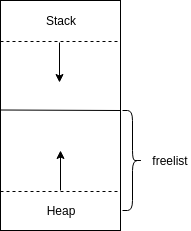
\includegraphics[scale=0.5]{memory}
    \end{center}
\end{frame}

\begin{frame}{Operational Semantics}
  \begin{itemize}
  \item Variables\; $\ms{Var} ::= x_1,x_2,...$
    \item Locations\; $\ms{Loc} ::= l_1,l_2,...$
    \item Values\; $\ms{Val} ::= \irl{T} ,\irl{F}, \mathbb{N}, \ms{Loc}, \pairexcst{v_1}{v_2} $
    \item Stacks: $\ms{Var} \to \ms{Val}$
    \item Heaps: $\ms{Loc} \to \ms{Val}$
    \end{itemize}

    \[V,H \vdash e \Downarrow v,H'\] Under stack $V$ heap $H$, $e$ evaluates to
    value $v$ and heap $H'$
\end{frame}
  
\begin{frame}{Reachability}
 

  \begin{mathpar}
\inferrule{
	A = reach_H(v_1)\\
	B = reach_H(v_2)
}{
	A \uplus B = reach_H(\pairexcst{v_1}{v_2}) 
} 

\inferrule{
	A = reach_H(H(l))\\
}{
	\{l\} \uplus A = reach_H(l)
} 

\inferrule{
	v \in \mathbb{N} \cup \{\irl{T},\irl{F},\irl{Null}\}
}{
	\emptyset = reach_H(v)
} 
\end{mathpar}

For a program state $(V, H,e)$, associate to it the \emph{reachable set}:
\begin{align*}
  &locs_{V,H}(e) = \biguplus\limits_{x \in FV(e)} reach_H(V(x))
\end{align*}
Cost of a program could be defined as the \emph{maximum} size of
the reachable set for any $(V,H,e)$ in execution. 
\end{frame}

\begin{frame}{Previous Work}
  \begin{itemize}
  \item Spoonhower, Blelloch, Harper: cost semantics for parallel programs
    \item Minamide: cost semantics for cbv lambda calculus
    \end{itemize}
  \end{frame}

\begin{frame}{Leaf Saturation +  Aggregation}
  Reachable at the leaf:
        \[
	\inferrule{
		V(x) = v
		}{
			V,H,R \vdash x \Downarrow^{|dom(R \uplus reach_H(v))|} v,H
			}
         \]
Aggregate:
\[
	\inferrule{
		V,H,R \uplus locs_{V,H}(x.e_2) \vdash e_1 \Downarrow^{s_1} v_1,H_1\\
		V[x \mapsto v_1],H,R \vdash e_2 \Downarrow^{s_2} v_2,H_2\\
	}{
		V,H,R \vdash \irl{let}(e_1; x : \tau.e_2) \Downarrow^{\max{s_1,s_2}} v_2,H_2
	}
      \]
      
  \end{frame}

\begin{frame}{Freelist}
  \begin{itemize}
  \item Problem: cost accounted for on use site instead of creation
  \item Solution: add persistency through freelists
  \end{itemize}
The garbage collection cost semantics \gcSem{} is defined by a collection of judgement of the form
\[
V,H,R,F \; \vdash e \Downarrow v, H', F'
\]

Under stack $V$, heap $H$, continuation set $R$,
freelist $F$,  the $e$ evaluates to  $v$, 
new heap $H'$ and freelist $F'$.
\end{frame}

\begin{frame}{Judgments}
\begin{mathpar}
\inferrule
{ V(x) = v\\
}
{V,H,R,F \; \vdash x \Downarrow v,H,F}(\text{Var})

\inferrule{
	V_1 = V\restriction_{FV(e_1)}\\
  R' = R \cup locs_{V,H}(\lambda x : \tau.e_2)\\
  V_1,H,R',F \vdash e_1 \Downarrow v_1,H_1,F_1\\
	V_2 = (V[x \mapsto v_1])\restriction_{FV(e_2)}\\
  g = \{ l \in H_1 \mid l \notin F_1 \cup R \cup locs_{V_2,H_1}(e_2) \}\\
  V_2,H_1,R, F_1 \cup g \vdash e_2 \Downarrow v_2,H_2,F_2 \\
}{
  V,H,R,F \; \vdash \irl{let}(e_1; x : \tau.e_2) \Downarrow v_2,H_2,F_2
}(\text{Let})
\end{mathpar}

\end{frame}


\section{Type System}

\begin{frame}{First Order Types}
  \[
\begin{array}{r l l l c r l l l}
  \ms{BTypes} & A \,\,\,\,\, ::= &\hspace{8em}     &  &\\
	& \irl{nat}                	 			& \irl{nat}										\\
	& \unittyabt                	 			& \unittycst								\\
  & \booltyabt                       & \booltycst                \\
              & \prodtyabt{A_1}{A_2}       & \prodtycst{A_1}{A_2}\\
  	&\irl{list}^p(A)		& L^p(A)\\

 \ms{FTypes} & \rho \,\,\,\,\, ::= \\
              &\irl{arr}(A_1;A_2;p;q) 				& A_1 \xrightarrow{p/q} A_2\\ 	
\end{array}
\]

Cost Model: only cons cells have a cost of 1, all other values have cost 0
\end{frame}

\begin{frame}{Structural Values}

\begin{align*}
	\denote{\unittyabt} &= \{\val{\irl{Null}}\}\\
	\denote{\booltyabt} &= \{\val{\irl{T}}, \val{\irl{F}}\}\\
	\denote{\irl{nat}} &= \mathbb{N}\\
\pairexcst{a_1}{a_2} &\in \denote{\prodtycst{A_1}{A_2}} 
	\text{ if } a_1 \in \denote{A_1} \text{ and } a_2 \in \denote{A_2}\\
\nilexcst &\in \denote{L(A)}\\
\consexcst{a}{l} &\in \denote{L(A)} \text{ if } a \in \denote{A} \text{ and } l \in \denote{L(A)}\\
\end{align*}
\end{frame}

\begin{frame}{Linear Potential}
\begin{align*}
	&\Phi_H(v : A) = 0 \text{ if } A \in \{\unittycst, \booltyabt, \irl{nat}\}\\
&\Phi_H(\pairexcst{v_1}{v_2} : \prodtycst{A_1}{A_2}) = \Phi_H(v_1 : A_1) + \Phi_H(v_2 : A_2)\\
	&\Phi_H(l : L^p(A)) = p + \Phi_H(v_h : A) + \Phi_H(v_T : L^p(A)) \text{ if } 
		H(l) = \pairexcst{v_h}{v_h}
	%p\cdot n + \sum_{1 \le i \le n} \Phi_H(a_i : A)  
\end{align*}
%
Write $\Phi_{V,H}(\Gamma)$ for $\Sigma_{x \in dom(V)} \Phi_H(V(x) : \Gamma(x))$.\\
Now define $A \curlyvee A_1,A_2$ as the sharing relation for resource-annotated types:
\begin{align*}
	&L^p(A) \curlyvee L^q(A_1),L^r(A_2) & \text{if } p = q + r \;\text{and}\; 
			A \curlyvee A_1,A_2\\
	&\prodtycst{A}{B} \curlyvee \prodtycst{A_1}{B_1}, \prodtycst{A_2}{B_2}
		&\text{ if } A \curlyvee A_1,A_2 \text{ and } B \curlyvee B_1,B_2\\
	&A \curlyvee  A,A& \text{ if } A \in \{\unittycst, \booltycst, \irl{nat}\}
\end{align*}
Enables ``quasi-linear'' type system that allows variable sharing
\end{frame}

\begin{frame}[fragile]{Example}
  \begin{verbatim}
let rec append (l1, l2) =
  match l1 with
  | [] -> l2
  | x::xs -> x::(append (xs, l2))

let appTwice l = 
    share l as l1,l2 in
    let l1' = append (l1, []) in 
    let l2' = append (l2, []) in 
    (l1',l2')

;;

let _  = append [1;2;3;4;5] [] in 
let _ = appTwice [1;2;3;4;5] in ()
  \end{verbatim}
\end{frame}

\begin{frame}[fragile]{Example}
  \begin{verbatim}
let rec append (l1, l2) =
  match l1 with
  | [] -> l2
  | x::xs -> x::(append (xs, l2))

let appTwice l = 
    share l as l1,l2 in
    let l1' = append (l1, []) in 
    let l2' = append (l2, []) in 
    (l1',l2')

;;

let _  = append [1;2;3;4;5] [] in (* overhead = 0 *)
let _ = appTwice [1;2;3;4;5] in () (* overhead = |l| = 5 *)
  \end{verbatim}
\end{frame}


\begin{frame}{Example}
  Notice that for \texttt{append}, the program is 
  \begin{itemize}
  \item completely linear
  \item cost can be accurately modeled by destructive pattern matching
  \end{itemize}
  For \texttt{appTwice}, the program is
  \begin{itemize}
  \item non-linear due to sharing
  \item destructive pattern matching is unsound
  \end{itemize}
  But we can still derive a reasonable bound for \texttt{appTwice} if the type system can 
  somehow treat shared variables in a linear way
\end{frame}

\begin{frame}{Old bounds}
  Currently, these are the best bounds derivable in RaML:
  \begin{align*}
	&\texttt{append} : \prodtycst{L^p(\irl{int})}{L^q(\irl{int})} \xrightarrow{r/r} L^s(\irl{int}), \text{ 
	where } p \ge s + 1 \text{ and } q \ge s\\
	&\texttt{appTwice} : L^p(\irl{int}) \xrightarrow{q/q} \prodtycst{L^r(\irl{int})}{L^s(\irl{int})},
	\text{ where } p \ge r + s + 2
\end{align*}

\end{frame}

\begin{frame}{Copy Sharing}
Destructive matching can be made sound if we introduce copy sharing:
\begin{align*}
	&L^p(A) \curlyvee^n L^q(A_1),L^r(A_2) & \text{if } p = q + r + n \;\text{and}\; 
			A \curlyvee^n A_1,A_2\\
	&\prodtycst{A}{B} \curlyvee^n \prodtycst{A_1}{B_1}, \prodtycst{A_2}{B_2}
		&\text{ if } A \curlyvee^n A_1,A_2 \text{ and } B \curlyvee^n B_1,B_2\\
	&A \curlyvee^n  A,A& \text{ if } A \in \{\unittycst, \booltycst, \irl{nat}\}
\end{align*}
Setting $n = 1$ gives the right copying overhead for the current cost model
\end{frame}

\begin{frame}{Type Rules}
  Now, destructive matching is sound:
  \begin{mathpar}
\inferr{
  \Sigma; \Gamma, x : L^p(A) \sststile{q'}{q} \listcaseexcst{x}{e_1}{x_h}{x_t}{e_2} : B
}{
  \Sigma; \Gamma \sststile{q'}{q} e_1 : B \\
  \Sigma; \Gamma, x_h : A, x_t : L^p(A) \sststile{q'}{q + p + {\color{red}{1}}} e_2 : B
}(\text{L:MatL})

\inferr{
  \Sigma; \Gamma, x : A \sststile{q'}{q} \sharecpcst{x}{x_1}{x_2}{e} : B
}{
  A \;\curlyvee^{\color{red}{1}} \;A_1, A_2\\
  \Sigma; \Gamma, x_1 : A_1, x_2 : A_2 \sststile{q'}{q} e : B
}(\text{L:Share})

  \end{mathpar}
\end{frame}

\begin{frame}{New Bounds}
  \begin{align*}
	&\texttt{append} : \prodtycst{L^p(\irl{int})}{L^q(\irl{int})} \xrightarrow{r/r} L^s(\irl{int}),
	\text{ where } {\color{green}{p \ge s}} \text{ and } q \ge s\\
	&\texttt{appTwice} : L^p(\irl{int}) \xrightarrow{q/q} \prodtycst{L^r(\irl{int})}{L^s(\irl{int})},
	\text{ where } p + q \ge r + s + {\color{green}{1}}
\end{align*}
\end{frame}

\begin{frame}[fragile]{Results}
\begin{table}[]
	\begin{adjustbox}{width=1\textwidth, center=\textwidth}
  \begin{tabular}{@{}llllllllll@{}}
    \toprule
		 & \multicolumn{3}{l}{heap metric} & \multicolumn{3}{l}{gc metric} &  \\ \midrule
		 \textit{\textbf{function}} & computed bound & constraints & time & computed bound &  constraints & time & optimal \\
		 quicksort & $1.00 + 3.50M + 1.50M^2$ & 8515 & 0.52 & 0 & 8519 & 0.48 & 0 \\
		 mergesort & $1.00 - 4.67M + 6.33M^2$ & 9572 & 0.64 & $-0.50M + 0.50M^2$ & 9578 & 0.58 & $\lfloor \log(M) \rfloor$ \\
		 ocamlsort & $7.50 + 5.50M + 1.00M^2$ & 8565 & 0.51 & $1.00 + 1.00M$ & 8573 & 0.50 & $M+1$ \\
		 selection sort & $2.00 + 3.00M + 1.00M^2$ & 639 & 0.06 & 0 & 642 & 0.05 & 0 \\
		 eratosthenes & $1.00 + 1.50M + 0.50M^2$ & 515 & 0.06 & 0 & 517 & 0.04 & 0 \\
		 dfs & $3.00 + 2.00M$ & 5481 & 0.90 & 2 & 5483 & 0.36 & 2 \\
		 bfs & $5.00 + 10.00M$ & 24737 & 4.15 & 4 & 24742 & 1.62 & 4 \\
		 transpose & $1.00 + 3.50LM + 0.50LM^2$ & 10680 & 0.50 & $1.00 + 2.00LM$ & 10684 & 0.50 & $\max{(0,2L-1)}$ \\
		 map\_it & $2.00 + 2.00LM + 4.00M$ & 30699 & 1.58 & $1.00M + 1.00$ & 30703 & 1.57 & M + 1 \\
		 pairs & $1.00 + 1.00M^2$ & 10214 & 0.60 & $0.50M + 0.50M^2$ & 10217 & 0.64 & $0.5M^2-1.5M+2$ \\ \midrule
	\end{tabular}
	\end{adjustbox}
	\caption{Automatic Bound Analysis with RaML}
\label{table:bounds}
\end{table}
\end{frame}


\section{Soundness}
\begin{frame}{Soundness}
\begin{theorem}[Soundness]
\label{itm:soundness} Let $H \vDash V {:} \Gamma$, $\;\; \Sigma; \Gamma \sststile{q'}{q} e : B$,
and $V,H \vdash e \Downarrow v, H'$.
Then for all configurations $W,Y,F,R$:
If $V,H \sim W,Y$ and $|F| \ge \Phi_{V,H}(\Gamma) + q$,
then there exists a value $w$, and a freelist $F'$ such that
$$
\begin{array}{ccc}
	W,Y,R,F \vdash^{\gcSem} e \Downarrow w, Y', F'  & \text{ and } & \veq{H'}{Y'}{v}{w} \; .
\end{array}
$$
\end{theorem}
The theorem states that,
given a terminating expression
and a freelist that is sufficiently large (as predicated by the type derivation), 
a run with \gcSem will normalize to an equivalent value.
\end{frame}

\begin{frame}{Proof Sketch}
  \begin{itemize}
  \item define an intermediate semantics \copySem{} which is semantically linear
  \item show \copySem{} over-approximates \gcSem
  \item show $\fogc$ is sound with respect to \copySem{}
  \end{itemize}
  i.e.

\tikzstyle{process} = [rectangle, text centered, draw=black, fill=orange!30]
\tikzstyle{arrow} = [thick,->,>=stealth]

\begin{center}
\begin{tikzpicture}[node distance=2cm]
\node (type) [process] {Type Rules};
\node (copy) [process, right of=type, xshift=3cm] {\copySem};
\node (free) [process, below of=copy] {\gcSem};

\draw [arrow] (type) -- node[anchor=south] {sound w.r.t (\ref{itm:soundness})} (copy);
\draw [arrow] (copy) -- node[anchor=west] {Over-approximates (\ref{itm:frugal})} (free);
\draw [dashed,->] (type) -- node[anchor=south] {} (free);

\end{tikzpicture}
\end{center}
\end{frame}

\begin{frame}{Linear Semantics}
  Variable sharing is achieved via \emph{copying}: semantic counterpart/justification for the sharing
  relation in the type system

{ \small \begin{mathpar}
	\inferr{
		H,v = copy(H,L,v)	
	}{
		v \in \{n,\irl{T},\irl{F},\irl{Null}\}
	}

	\inferr{
		H'\{l' \mapsto v\},l' = copy(H,L,l) 
	}{
		l' \in L\\
		H',v = copy(H,L \setminus \{l'\},H(l)) 
	}

\inferr{
	H_2,\pairexcst{v_1'}{v_2'} = copy(H,L,\pairexcst{v_1}{v_2})
}{
	L_1 \sqcup L_2 \subseteq L\\
	|L_1| = |dom(reach_H(v_1)|\\
	|L_2| = |dom(reach_H(v_2)|\\
	H_1,v_1' = copy(H,L_1,v_1)\\
	H_2,v_2' = copy(H_1,L_2,v_2)\\
}
\end{mathpar}}
\end{frame}

\begin{frame}{Copy Sharing}
  \small \[
\inferrule{
	V(x) = v'\\
  L \subseteq F\\
  |L| = |dom(reach_H(v'))|\\
  H',v'' = copy(H,L,v')\\
	V' = (V[x_1 \mapsto v',x_2 \mapsto v'']) \restriction_{FV(e)}\\
	F' =	F \setminus L\\
	g = \{l \in H \mid l \notin F' \cup R \cup locs_{V',H}(e)\}\\
 	V',H',R,F' \sqcup g \; \vdash e \Downarrow v,H'',F''
}{
  V,H,R,F \; \vdash \sharecpcst{x}{x_1}{x_2}{e} \Downarrow v,H'',F''
}
\]
\end{frame}

\begin{frame}{Proof Attempt}
  \begin{attempt}
	Let $\mathcal{C}_2 = (V,H,R,F)$ be a configuration and $(\mathcal{C}_2, e)$ 
	be a linear computation. Given that 
	$\mathcal{C}_2 \vdash^{\mathsf{copy}} e \Downarrow v,H',F'$, 
	for all configurations $\mathcal{C}_1 = (W,Y,R,M)$ such that $W,Y \sim V,H$ and $|M| = |F|$,
there is exists a triple
$(w,Y',M') \in \ms{Val} \times \ms{Heap} \times \ms{Loc}$ such that
	\begin{center}
			$\mathcal{C}_1 \vdash^{\mathsf{free}} e \Downarrow w,Y',M'$
		and 	 $\veq{H'}{Y'}{v}{w}$
		and 	 $|M'| \ge |F'|$ .
	\end{center}
\end{attempt}
\end{frame}

\begin{frame}{Contention}
Induction on the derivation of the judgment in \copySem: trouble in E:Let. 
IH on first premise:
%
\begin{center}
	 $W_1,Y,R',M \vdash^{\mathsf{free}} e \Downarrow w_1,Y_1,M_1$ and, $\veq{H_1}{Y_1}{v_1}{w_1}$
         and,  $|M_1| \ge |F_1|$
\end{center}
%
To instantiate IH on the second premise, NTS $|M_1 \cup j| \ge |F_1 \cup g|$,
where $j$ is the set of collected locations in 
the \gcSem{} judgment. We cannot show this precisely because $g$ might contain more cells 
then $j$ due to the linearity of \copySem{}, thus preventing a piecewise comparison. 
But of course $|j|$ is always less than $|g|$, since \gcSem{} doesn't copy to share 
values! This shows that there is a mismatch between the induction hypothesis and the relationship
between the sizes of the respective freelists and the garbage sets. 

\end{frame}

\begin{frame}{\copySem{} over-approximates \gcSem}
  Idea: maintain a mapping $\gamma$ from the active heap used in the GC semantics
  $H_{gc}\setminus F_{gc}$ to \emph{subsets} of
the heap used in the copying semantics $H_{copy} \setminus F_{copy}$ such that the image of 
$H_{gc}\setminus F_{gc}$ under $\gamma$ forms a partition on $H_{copy} \setminus F_{copy}$.
The intuition is that given a cell $l \in H_{gc}$, there must be multiple cells
$\gamma(l)$ in  $H_{copy}\setminus F_{copy}$  
that are were allocated during sharing, and thus ``morally the same'' as $l$.

\begin{center}
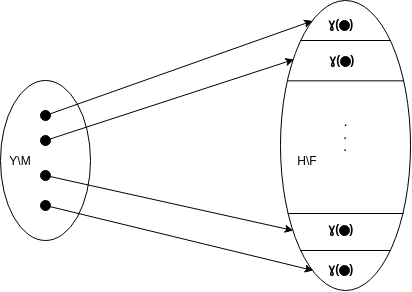
\includegraphics[scale=0.4]{relation}
\end{center}
\end{frame}

\begin{frame}{Well-formed configuration}
  \begin{definition} A configuration $(V,H,R,F)$ is well-formed if 
	\begin{enumerate}
		\item $dom(H) \subseteq reach_H(V) \cup R \cup F$
		\item $reach_H(V) \cup R \subseteq dom(H) \setminus F$
		\item $collect(R,reach_H(V),H,F) = \emptyset$
	\end{enumerate}
\end{definition}
\end{frame}

\begin{frame}{Subvalues}
  \begin{definition}
	Let \ms{dir} be the set \{\ms{L},\ms{R},\ms{N}\}, denoting left, right, and next 
	respectively. We can index values via directions:
        $$
	\begin{array}{lclclcl}
		get_H(Just(\pairexcst{v_1}{v_2},\ms{L})) &=& Just(v_1) & \hspace{4em} &
		get_H(Just(\pairexcst{v_1}{v_2},\ms{R})) &=& Just(v_2)\\
		get_H(Just(\pairexcst{v_1}{v_2}),_) &=& None &&
		get_H(Just(l),\ms{N}) &=& Just(H(l)) \\
		get_H(Just(l), \_) &=& None &&
		get_H(r,\_) &=& r
	\end{array}
        $$
	Let $P$ be a sequence of directions. Extend $get$ to sequence of directions:
	\begin{align*}
		find_H(v,D::P) &= find_H(get_H(v,D),P)\\
		find_H(v,[]) &= v
	\end{align*}
	Call $P$ valid w.r.t a value $v$ if $find_H(v,P) = Just (v')$ for some $v'$.
	Write $V_H(x;P)$ for $fromJust(find_H(V(x),P))$ given a valid sequence $P$ w.r.t $V(x)$,
	and $reach_H(V(x;P))$ for $reach_H(V_H(x;P))$.
\end{definition}
\end{frame}


\begin{frame}{Copy Extension}
\begin{definition}
A well-formed configuration $\mathcal{C}_2 = (V_2,H_2,R_2,F_2)$ is a \emph{copy extension} of another well-formed configuration
$\mathcal{C}_1 = (V_1,H_1,R_1,F_1)$ iff
\begin{enumerate}
\item $V_1,H_1 \sim V_2,H_2$
\item There is a proper partition $\gamma : dom(H_1) \setminus F_1 \to \mathcal{P}(dom(H_2) \setminus F_2)$ 
such that for all $l \in dom(\gamma)$, $|\gamma(l)| = reach_{H_1}(V_1)(l) + R_1(l)$
\item For all $l \in dom(\gamma)$, $x \in dom(V_1)$, valid sequence of directions $P$ w.r.t $V_1(x)$,
	$|reach_{H_2}(V_2(x;P)) \cap \gamma(l)| = reach_{H_1}(V_1(x;P))(l)$.
\item	For all $l \in dom(\gamma)$, $|\gamma(l) \cap R_2| = R_1(l)$
\item $|F_1| = |F_2| + |\oh{\gamma}|$, where 
	$\oh{\gamma} = \bigcup_{P \in ec(\gamma)} P \setminus (rep(P))$
\end{enumerate}
Write this as $\mathcal{C}_1 \preceq \mathcal{C}_2$.
\end{definition} 

The intention is that $\mathcal{C}_2$ is a configuration for initiating an evaluation using \copySem
, and $\mathcal{C}_1$ a configuration for \gcSem. 
\end{frame}

\begin{frame}{Extension Lemma}
  \begin{lemma}\label{itm:frugal}
	Let $(\mathcal{C}_2,e)$ be a linear computation. Given that 
	$\mathcal{C}_2 \vdash^{\copySem} e \Downarrow v,H',F'$,
	for all well-formed configurations $\mathcal{C}_1$ such that $\mathcal{C}_1 \preceq \mathcal{C}_2$,
there is exists a triple
$(w,Y',M') \in \ms{Val} \times \ms{Heap} \times \ms{Loc}$ and 
	$\gamma' : dom(Y') \setminus M' \to \mathcal{P}(dom(H') \setminus F')$ s.t.
	\begin{enumerate}
			\item $\mathcal{C}_1 \vdash^{\gcSem} e \Downarrow w,Y',M'$
			\item $\veq{H'}{Y'}{v}{w}$
			\item $\gamma'$ is a proper partition, such that for all $l \in dom(\gamma')$, 
				$|\gamma'(l)| = |reach_{Y_1}(w_1)(l)| + S(l)$
			\item For all $P$, $|reach_{H'}(find_{H'}(v;P)) \cap \gamma'(l)| = 
				reach_{Y'}(find_{Y'}(w;P))(l)$
			\item For all $l \in dom(\gamma')$, $\gamma'(l) \cap R = \gamma(l) \cap R$
			\item $|M'| = |F'| + |\oh{\gamma'}|$
	\end{enumerate}
\end{lemma}
\end{frame}



\begin{frame}{Linearity of \copySem}
\begin{definition}[Linear computation]
  Given a context $(V,H)$, let
$x,y \in dom(V)$, $x \ne y$, and $r_x = reach_H(V(x))$, $r_y = reach_H(V(y))$.
It is \emph{linear} given that  $\ms{set}(r_x)$, $\ms{set}(r_y)$, and $r_x \cap r_y = \emptyset$.
Given a configuration $\mathcal{C} = (V,H,R,F)$ and an expression $e$, 
we say the 5-tuple $(\mathcal{C},e)$ is a \emph{computation}; it is a \emph{linear computation} 
given the that  $dom(V) = FV(e)$, $\na{V,H}$, and $\dist{\{R,F,locs_{V,H}(e)\}}$.
Write $\wfc{V}{H}{R}{F}{e}$ to denote this fact.
\end{definition}

% main lemma
Given a semantically linear computation, the resulting value is linear: 
\begin{lemma}[Linearity of \copySem]\label{itm:na}
For all stacks $V$ and heaps $H$, let  $V,H,R,F \; \vdash e \Downarrow v, H', F'$ 
and $\Sigma; \Gamma \vdash e : B$. Then given that $\wfc{V}{H}{R}{F}{e}$, we have that $\ms{set}(reach_{H'}(v))$ and $\dist{\{R,F',reach_{H'}(v)\}}$.
\end{lemma}
\end{frame}

\begin{frame}{Operational Semantics}
  Let be $\mathcal{E}_{\ms{oper}}$ the normal operational semantics with
  rules of the form $V,H \vdash e \Downarrow v,H$.\\
  
  In words, the theorem states that given a terminating expression (as shown by a run with
  $\mathcal{E}_{\ms{oper}}$),
and given a freelist that is sufficiently large (as predicated by the type derivation), 
a run with \copySem will normalize to an equivalent value, and the resulting freelist 
will be sufficiently large (as predicated by the type derivation).
\end{frame}

\begin{frame}{Soundness of \copySem}
\begin{theorem}[Soundness]
\label{b} let $H_o \vDash V_o : \Gamma$, $\Sigma; \Gamma \sststile{q'}{q} e : B$,
$V_o,H_o \; \vdash e \Downarrow v_o, H_o'$.
Then $\forall C \in \mathbb{Q}^{+}$ and configuration $V,H,R,F$ s.t.
\begin{enumerate} 
\item $V_o,H_o \sim V,H$
\item $\wfc{V}{H}{R}{F}{e}$
\item $|F| \ge \Phi_{V,H}(\Gamma) + q + C$ 
\end{enumerate}
then there exists a triple $(v,H',F')$, and a freelist $F'$ s.t.
\begin{enumerate}
  \item $V,H,R,F \vdash^{\copySem} e \Downarrow v, H', F'$
	\item $\veq{H_o'}{H'}{v_o}{v}$
  \item $|F'| \ge \Phi_{H'}(v:B) + q' + C$
\end{enumerate}
\end{theorem}
\end{frame}

  
% Placing a * after \section means it will not show in the
% outline or table of contents.
\section*{Summary}

\begin{frame}{Summary}
  \begin{itemize}
  \item New cost semantics for garbage collection of first-order functional programs
  \item Extension of type based amortized analysis to derive better space bounds
  \item Soundness Theorem
  \end{itemize}
  
  \begin{itemize}
  \item Questions:
    \begin{itemize}
    \item Extension to higher-order functions
    \item Type rules for accounting for non-local garbage collection;
      variable sharing vs context sharing
    \end{itemize}
  \end{itemize}
\end{frame}



% All of the following is optional and typically not needed. 

\end{document}


